\documentclass[10pt,norsk,a4paper]{article}
\usepackage[utf8]{inputenc}
\usepackage[T1]{fontenc}
\usepackage[norsk]{babel}
\usepackage[cm]{fullpage}
\usepackage{color}
\usepackage{parskip,textcomp,amssymb,graphicx}
\usepackage{pdfpages}
\usepackage[stable]{footmisc}


\title{Generalforsamling \\
	Høsten 2017\\
	Cybernetisk Selskab\\[2cm]
	
\includegraphics[width=0.5\textwidth]{cyblogoa3.pdf}\\[-.5cm]}
\date{15.\ november 2017}

% Blank header, samt footer med side x av y
\usepackage{fancyhdr}
\pagestyle{fancy}
\renewcommand{\headrulewidth}{0pt}
\fancyhead{}
\cfoot{Side~\thepage\ av~\pageref{lastpage}}



\begin{document}

\maketitle{}
\newpage

\tableofcontents{}



\section{Valg av møteleder}

\section{Valg av referent}

\section{Valg av protokollunderskrivere}

\section{Valg av tellekorps}

\section{Godkjenning av innkalling}

\section{Godkjenning av dagsorden}

\section{Semesterberetninger}
\subsection{Semesterberetning ved leder}

\begin{quote}
	Kjære interne, medlemmer og studenter,

Dette har vært et bra år for Cybernetisk Selskab. Vi utvidet fadderuka i år, noe som ble en braksuksess. Vi arrangerte storfester de tre siste dagene av fadderuka, og vi hadde fortsatt ikke kapasiteten vi trengte. Selv om det er kjipt med kø, er det veldig postitivt at vi klarer å tiltrekke oss så mange studenter.

De to andre store arrangementene vi har holdt dette semesteret---dagen@ifi og Ifi-galla---gikk begge uten store problemer. Spesielt dagen@ifi virker det som om at vi har funnet en fin formel på hvordan vi skal arrangere dette sammen med dagen-styret.

Vi har også dette semesteret startet med en ny type arrangement: \textit{Torsdagsklubben / spritkveld}. Dette er et konsept som har slått bra an. Det er ikke fult hus på disse kveldene, men det kommer mer enn nok folk til at dette er et konsept vi burde fortsette med.

Personlig har jeg jobbet en del med det pågående prosjektet med å anskaffe nytt kassaapparat. Planen er per dags dato at denne vil bli installert første eller andre uken i desember, og at det blir tatt i bruk etter nyttår. Dette vil medføre enklere økonomirutiner, mindre teknisk kompleksitet, og at de interne i baren får noe nytt å leke med.

Medlemsmassen vår er på ca det samme som det var i fjor, med 714 semestermedlemmer, noe som vi kan si oss fornøyde med når vi tenker på at vi satte rekord i fjor.

Andreas Hansen,\\
leder
\end{quote}

%\newpage


\subsection{Semesterberetning ved kjellermogul}

Karl H. Totland orienterer med semesterberetning enten lagt inn som vedlegg under generalforsamlingen \textit{eller} ved oppdatering før generalforsamlingen.

%\newpage

\section{Kasserer orienterer}
\subsection{Regnskapets tilstand}
Kasserer orientere om regnskapet.


\subsection{Revidert budsjett for høsten 2017}
Kasserer orientere om budsjett.



\section{Kontigentfastsettelse}
Hovedstyret foreslår å endre medlemskontigenten fra kr. 30,- til kr. 40,-,
fra og med neste semester. \\
Hovedstyret orienterer rundt motivasjonen bak dette.


\section{Valg}

\begin{minipage}[t]{9cm}
\subsection{Hovedstyret}
Man velges inn i hovedstyret for ett år av gangen.

\subsubsection{Kjellermogul}
\subsubsection{Kasserer}
\subsubsection{Arrangementssjef}
\subsubsection{Promoteringssjef}
\subsubsection{Internansvarlig}

\end{minipage}
\begin{minipage}[t]{9cm}
\subsection{Kjellerstyret}
Alle verv--\textit{utenom økonomiansvarlig}--som er til valg i \\kjellerstyret gjelder for ett semester av gangen.

\subsubsection{Økonomiansvarlig}
\subsubsection{Innkjøpsansvarlig}
\subsubsection{Barsjef}
\subsubsection{Kafésjef}
\subsubsection{Teknisk ansvarlig}
\subsubsection{DJ-sjef}
\subsubsection{Utlånsansvarlig}
\subsubsection{Arrangementskoordinator\footnotemark}

\end{minipage}
\footnotetext{Tentativ vervtittel.}

\newpage

\section{Vedtektsendringer}
Følgende forslag til vedtektsendringer ligger fremme.

\subsection{Endring i forbindelse med krav om Ifi-foreninger}

For å være en offisiell Ifi-forening har Ifi satt sammen noen vedtekter som studentforeningene må følge. 
Per dags dato følger ikke Cybernetisk Selskab §1c\footnotemark. Det ble lagt frem et forslag av hovedstyret på vårens generalforsamling om å endre våre vedtekter, slik at vi ikke bryter med Ifi sine krav. 
Dette ble da ikke vedtatt da forsamlingen konkludere med at de nye vedtektene var for åpne og uklare. Forsamlingen ønsket at hovedstyret skulle komme med et nytt forslag til neste generalforsamling, som blir denne, høsten 2017.

\footnotetext{Etter manglende vedtektsfesting av to-tredelers Ifi-studenter i hovedstyret}

Om vedtektene ikke blir vedtatt vil hovedstyret starte søknadsprosessen for å få et unntak fra §1c av \textit{Vedtekter for Ifi-forening}, slik som §3c åpner for. Begge endringsforslagene hører sammen og stemmes over i lag.

Hovedstyret er innstilt på å starte søknadsprosessen etter §3c.

\subsubsection{Forslag til ny paragraf: $§5h$}
\begin{quote}
	\begin{enumerate}
		\item[§5h] Minimum to-tredeler av hovedstyret skal bestå av studenter som enten (1) er tilknyttet et eller flere studieprogrammer ved \textit{Institutt for informatikk}, eller (2) som tar ett eller flere IN- eller INF-fag.
	\end{enumerate}
\end{quote}

\subsubsection{Forslag til endring av paragraf: §8a}
\begin{quote}
	\begin{enumerate}
		\item[§8a] 
			Valgbare til alle styrer er alle medlemmer i henhold til §2 og informatikkstudenter ved Universitetet i Oslo. \textcolor{red}{Om valg av kandidat bryter med §5h, blir valget gjort ugyldig og det blir gjenvalg. Om ingen andre kandidater stiller blir vervet etterfylt av hovedstyret i henhold til §5f.} Alle valg avgjøres \textcolor{red}{på generalforsamling} ved simpelt flertall.
	\end{enumerate}
\end{quote}


\section{Æresmedlemskap}

\section{Utdeling av pins}
Arkivar deler ut pins.

\section*{Vedlegg: Cybernetisk Selskabs vedtekter}
\section*{Vedlegg: Vedtekter for Ifi-foreninger}\label{lastpage}


\newpage

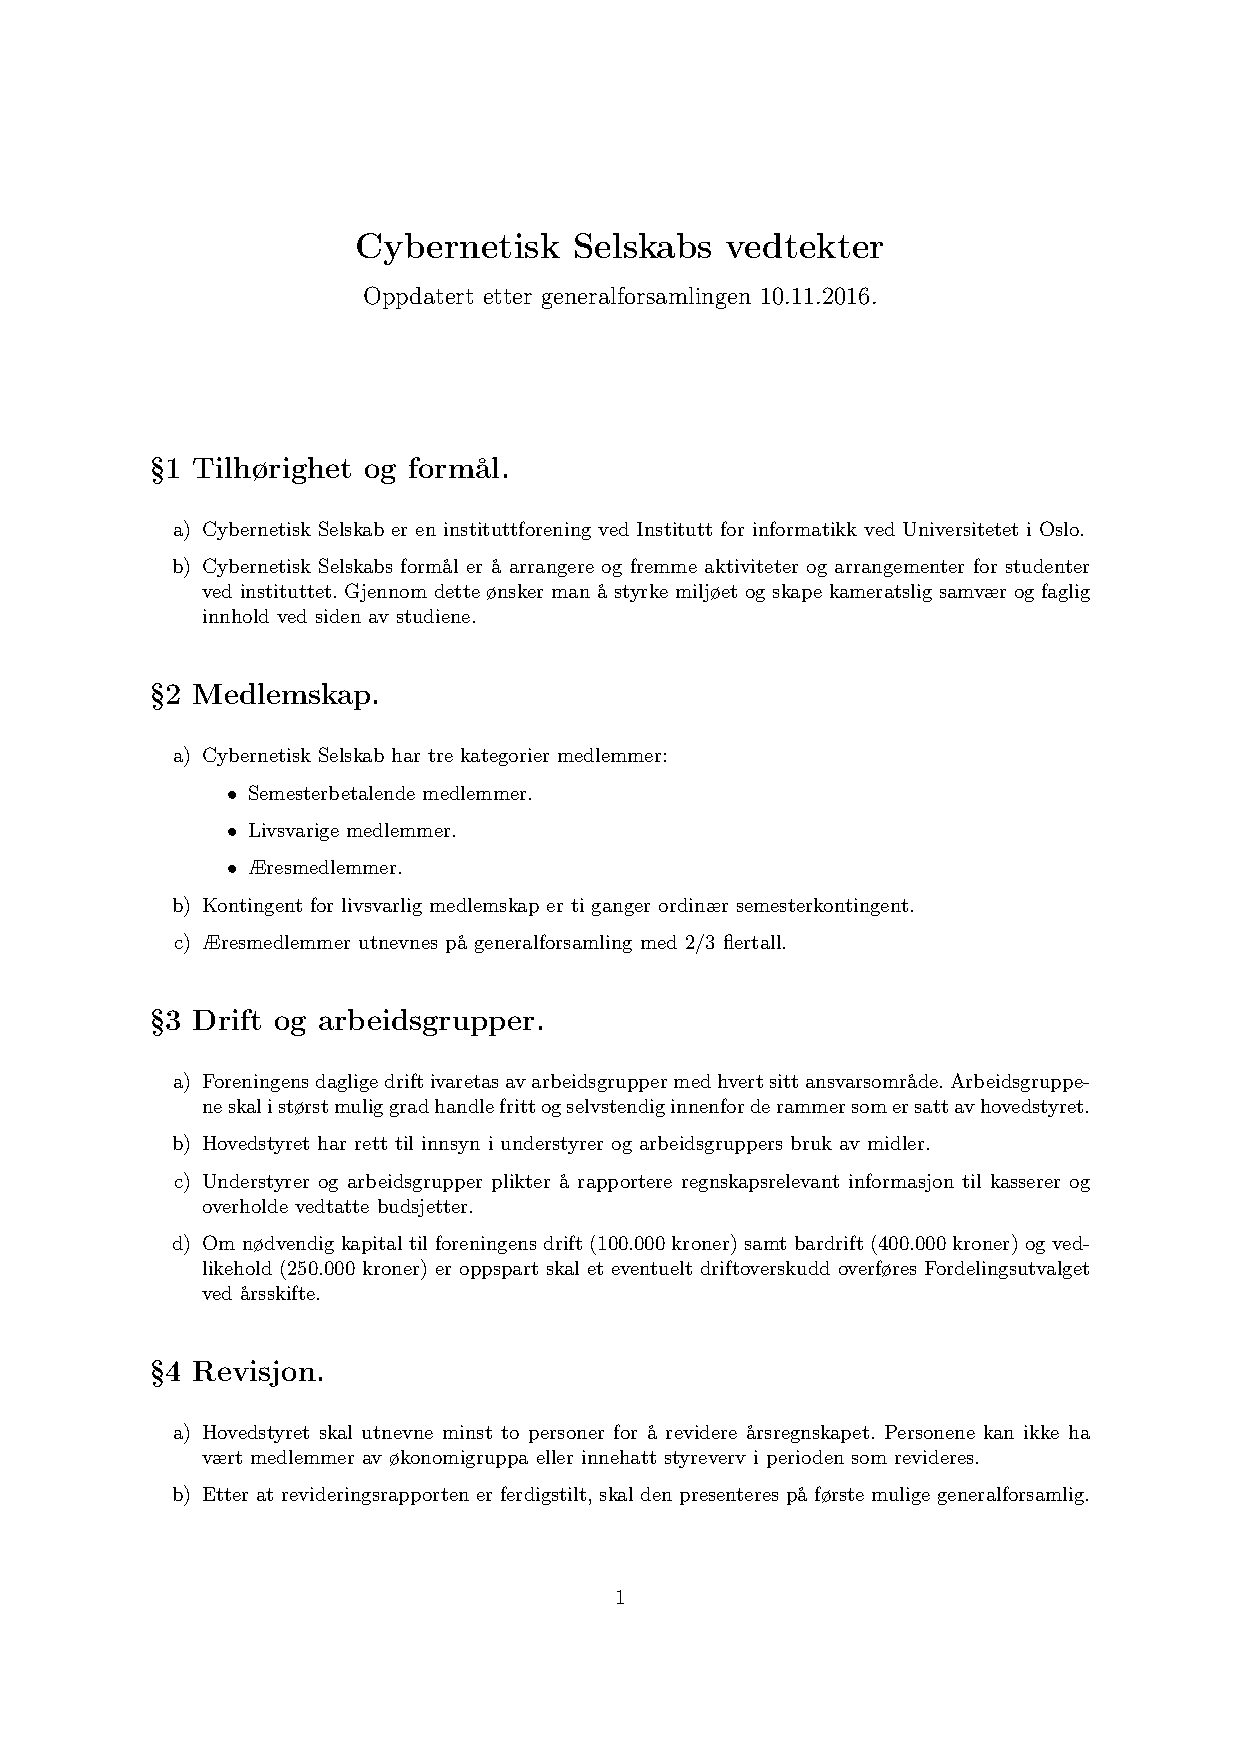
\includepdf[pages=-]{cyb_vedtekter.pdf}
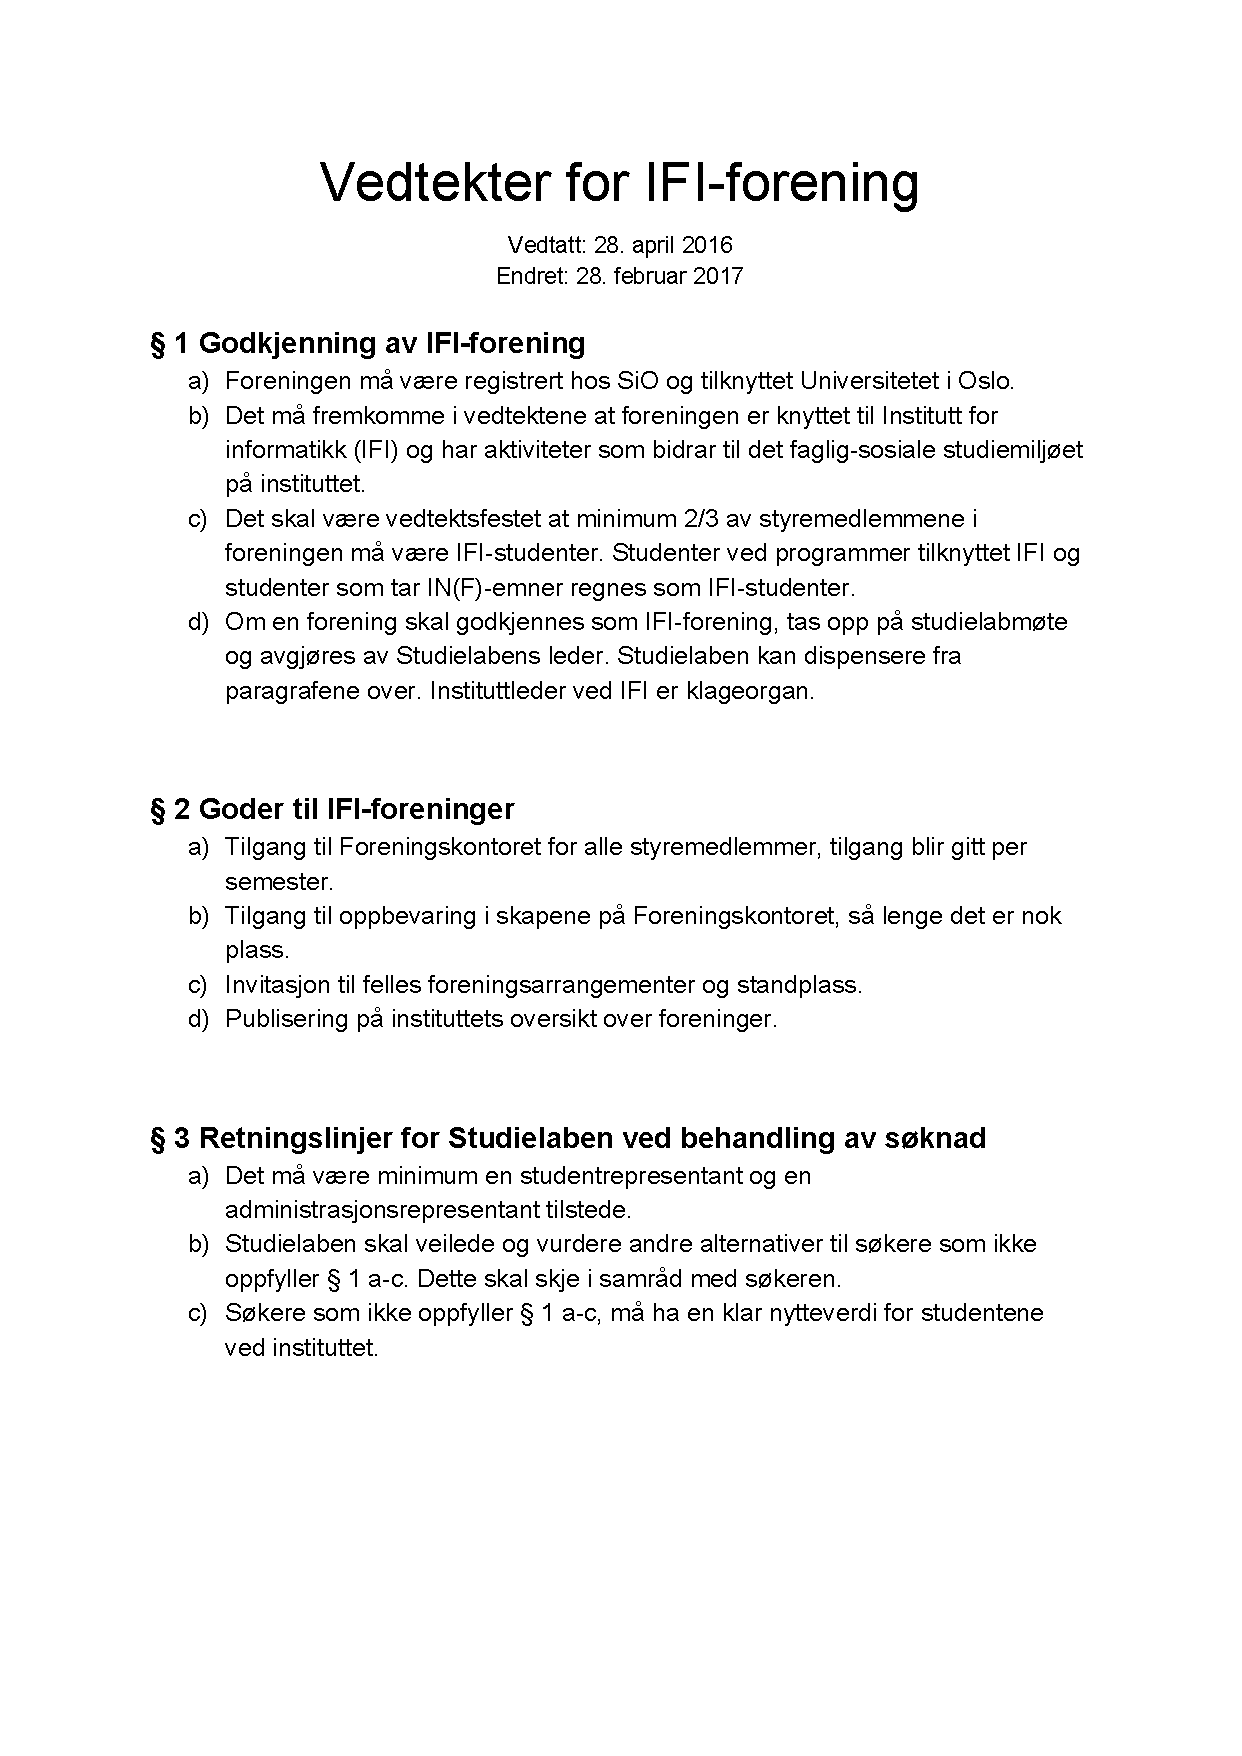
\includepdf[pages=-]{ifi_forening_vedtekter_2017.pdf}
\end{document}
